%%%Écrit par Jean-Raphaël Carrier en collaboration avec Claudine Allen%%%
%Dernière modification JRC: 10 janvier 2014
%Dernière modification CA: 15 janvier 2024
%
%**ToDo**: 
% - Voir si je recopie ou déplace les instructions de transfert de fichiers sur Teams et OneDrive dans le premier laboratoire au lieu de lab suivants. (P-e déjà fait).
% - Spécifier qu'on peut enrouler les fils du module directement autour des électrodes au départ, en dégainant plus au besoin: mentionner leur pince à dégainer. Expliquer en mode "conception" quand rendus à l'utilisation de plaquette de montage référant au fil & pinces introduits en vidéo : - Comment faire son circuit à la patate (banane + croco qui ne devrait pas servir après!) - Comment brancher mutimètre (fil multi + pince grabber), etc. et nous consulter pour apprendre et optimiser.
%- Plus d'analyse statistique: rapport signal/bruit, tester la propagation d'incertitude à partir de distribution complète vs ses moments comme variance vs min-max, etc.
%- Pour le complément associé, focaliser plutôt sur les concepts de résolution en acquisition numériques ainsi que rapport signal-bruit pour renvoyer au document métro & stats. 
%
\RequirePackage[l2tabu, orthodox]{nag} %Check for obsolete commands
\documentclass[canadien,12pt,oneside,letterpaper]{article}
%
%-----------------------------------------------------
%Loading packages
%
\usepackage[utf8]{inputenc}
\usepackage[T1]{fontenc}
\usepackage{babel}
\usepackage{lmodern}
\usepackage{textcomp}
\usepackage{amsmath,amssymb}
\usepackage{siunitx}
\usepackage{xcolor}
\PassOptionsToPackage{hyphens}{url}\usepackage[colorlinks=true,allcolors=blue]{hyperref}
\usepackage[all]{hypcap}
\usepackage{graphicx}
\usepackage[oldvoltagedirection,americanvoltages,americancurrents,siunitx]{circuitikz}
\usetikzlibrary{babel}
\usepackage{caption}
\usepackage{enumitem}
\usepackage[letterpaper,headheight=15pt]{geometry}
\usepackage{fancyhdr}
\usepackage{setspace}
%
%----------------------------------------------------
%Other configurations and layout
%
\sisetup{separate-uncertainty,locale=FR}
\captionsetup{font=small,labelfont=bf,margin=0.1\textwidth}
\newlist{gradescope}{enumerate}{2}
\setlist[gradescope,1]{label=Q\arabic{gradescopei},leftmargin=36pt,labelsep=18pt}
\setlist[gradescope,2]{label=Q\arabic{gradescopei}.\arabic{gradescopeii},leftmargin=-2pt,labelsep=8pt}
\pagestyle{fancy}
\fancyhf{}
\lhead{\textsl{GPH-2006/PHY-2002~---~Laboratoire~I}}
\rhead{\textsl{Page \thepage}}
\setcounter{secnumdepth}{0}
\setlength{\parskip}{1.5ex plus0.5ex minus0.2ex}
%\onehalfspacing
\interfootnotelinepenalty=10000 %To avoid footnotes spreading on several pages.
%
%---------------------------------------------------
%
\title{\vspace{-1.8cm}\textbf{Laboratoire I}\\Métrologie \& statistiques : acquisition numérique\thanks{Auteurs: Claudine Allen, Jean-Raphaël Carrier \& Annie-Claude Parent}}
\renewcommand\footnotemark{}
\date{}

\begin{document}

\maketitle \vspace{-1.8cm}

\noindent\textit{\textbf{Prélude de structure et logistique des laboratoires}} \par
\textit{Chaque protocole est divisé en 5 sections qui, à l'exception des \nameref{sec:obj} et du \nameref{sec:mat}, correspondent au moment où le travail de laboratoire doit être effectué:}\par
\begin{itemize} \itshape
    \item \nameref{sec:prep} $\rightarrow$ avant la séance de laboratoire,
    \item \nameref{sec:manip} $\rightarrow$ pendant, en parallèle avec l'expérimentation,
    \item \nameref{sec:grade} $\rightarrow$ après, dans la semaine qui suit.
\end{itemize}
\vspace{0.5ex}
\noindent{\itshape La recherche en science et génie va donc bien au-delà de faire les expériences proprement dites et le \texttt{Cahier de recherche} est votre journal de bord pour vous accompagner à toutes ces étapes. N'hésitez pas à y écrire vos pensées en tout temps dans le cahier OneNote de votre équipe <\url{https://www.onenote.com/notebooks}>, surtout en ce premier cours de laboratoire où son évaluation se concentre beaucoup sur la consignation de la recherche en temps réel. La rédaction du cahier selon les consignes du guide, qui assure la traçabilité et la continuité de la recherche, sera donc notée sur la base d'une auto-évaluation collaborative cette session en vue de progresser vers une évaluation complète dans les cours expérimentaux subséquents.
\vspace{1.5ex}

La compréhension du contenu en laboratoire sur l'électronique, la métrologie, l'analyse des résultats et la statistique, quant à elle, repose sur une évaluation des \nameref{sec:prep} (quiz sur le site de cours) et des \nameref{sec:grade} (énoncées à la fin du protocole et à remettre sur <\url{https://www.gradescope.com/}>). La toute dernière de celles-ci suivra votre progression en rédaction scientifique et technique sur les 4 premiers laboratoires qui, en rassemblant les réponses, forment l'essentiel de votre premier rapport de laboratoire universitaire. Du côté des lectures, elles constituent la première étape pour bien se préparer à toute séance de recherche en laboratoire, puisqu'il faut bien sûr comprendre le sujet des expériences que l'on veut développer. Un.e chercheur.e professionnel.le doit trouver des sources rigoureuses sur le sujet en étant de préférence assisté.e par le service d'une bibliothèque scientifique pour exercer un jugement critique sur la qualité des sources dans la surabondance d'informations en ligne. Une bonne préparation expérimentale se complète alors comme un.e athlète qui se prépare pour un match sportif, soit en visualisant et calculant d'avance tout ce qui pourrait se produire au laboratoire.}

\section{Objectifs} \label{sec:obj}

Ce laboratoire vise à familiariser l’étudiant à l’acquisition de données assistée par ordinateur, en particulier pour la caractérisation d’un système instable où la variation de la grandeur mesurée rend impraticable l’utilisation d’un instrument avec afficheur numérique ou analogique. En plus d’introduire les premières notions de base en métrologie et analyse statistique, ce laboratoire met ainsi l’accent sur une situation plus typique de la recherche expérimentale au lieu du cadre didactique habituel. L’étudiant sera sensibilisé à l’importance de choisir une méthode de mesure et de présentation des résultats appropriée à l’expérience ainsi qu’à la pertinence de l’analyse qualitative. 

%Les travaux effectués aborderont les objectifs d’ensemble 1, 2, 6, 7, 9, 10 et 11 du plan de cours et couvriront la qualité 5~--~utilisation d’outils d’ingénierie, prescrite dans les normes du Bureau d'agrément d'Ingénieurs Canada (BAIC).
%\thispagestyle{empty}
%\newpage

\section[Lectures préparatoires]{Lectures préparatoires\footnote{Accédez le quiz sommatif pour ces lectures sur le site de cours, en arrivant à chaque laboratoire.}} \label{sec:prep}
\vspace{-2ex}

\begin{itemize} \itemsep3pt
\item le manuel\footnote{\label{airtable}Tous les manuels d'instruction se retrouvent dans la colonne correspondante de la liste d'inventaire des composants \& instruments à l'adresse <\url{https://airtable.com/shrdI8Y6AqbNd7tZ8}>.} du module d'acquisition (pages 1 à 3, 12 à 15 et 24 à 26);
\item le manuel\textsuperscript{\footnotemark\ref{airtable}} du multimètre à 4\textonehalf~chiffres (pages 20 à 24); 
\item le manuel\textsuperscript{\footnotemark\ref{airtable}} du multimètre à 6\textonehalf~chiffres (pages 17 à 22);
\item le complément \textit{Introduction à LabVIEW}, l'annexe n'est pas obligatoire, mais pourra vous être fort utile en cas de problème(s) de communication avec les instruments;
\item le complément \textit{Fonctionnement d'une pile électrochimique};
\item les sections "Introduction" et "Conclusion" du \textit{Guide de rédaction de rapports scientifiques};
\item le protocole de ce laboratoire en portant une attention particulière à la section \nameref{sec:grade}: à la sortie de chaque séance, il faut s'assurer d'avoir toutes les données correctes et autres informations nécessaires pour répondre à ces questions.
\end{itemize}
\vspace{1ex}
\noindent\framebox{\parbox{\dimexpr\linewidth-2\fboxsep-2\fboxrule}{En plus de ces lectures, n'hésitez pas à noter vos réflexions et avancer votre préparation dans le cahier de recherche, allant du calcul de valeurs de référence à des tableurs pour recevoir vos données et leurs incertitudes, etc. Il est aussi recommandé de débuter la programmation des VI \textit{LabVIEW} puisque le temps nécessaire varie en fonction de votre pratique et des bogues!}}

%\vspace{1ex}
% \noindent\framebox{\parbox{\dimexpr\linewidth-2\fboxsep-2\fboxrule}{Cette dernière étape de préparation, pour vous familiariser avec le service logiciel Tinkercad, doit être faite en ligne INDIVIDUELLEMENT par tous.tes.}}

% Veuillez d'abord rejoindre votre compte de classe ici <\url{https://www.tinkercad.com/joinclass/QH1RQQYNCB5K}> à l'aide de votre IDUL comme \texttt{nickname} pour vous retrouver sur votre \texttt{Dashboard}. Si ce n'est pas le cas, vous devriez pouvoir y retourner en tout temps en cliquant sur le logo carré multicolore de Tinkercad.
% %
% \begin{figure}[h]
%     \centering
%     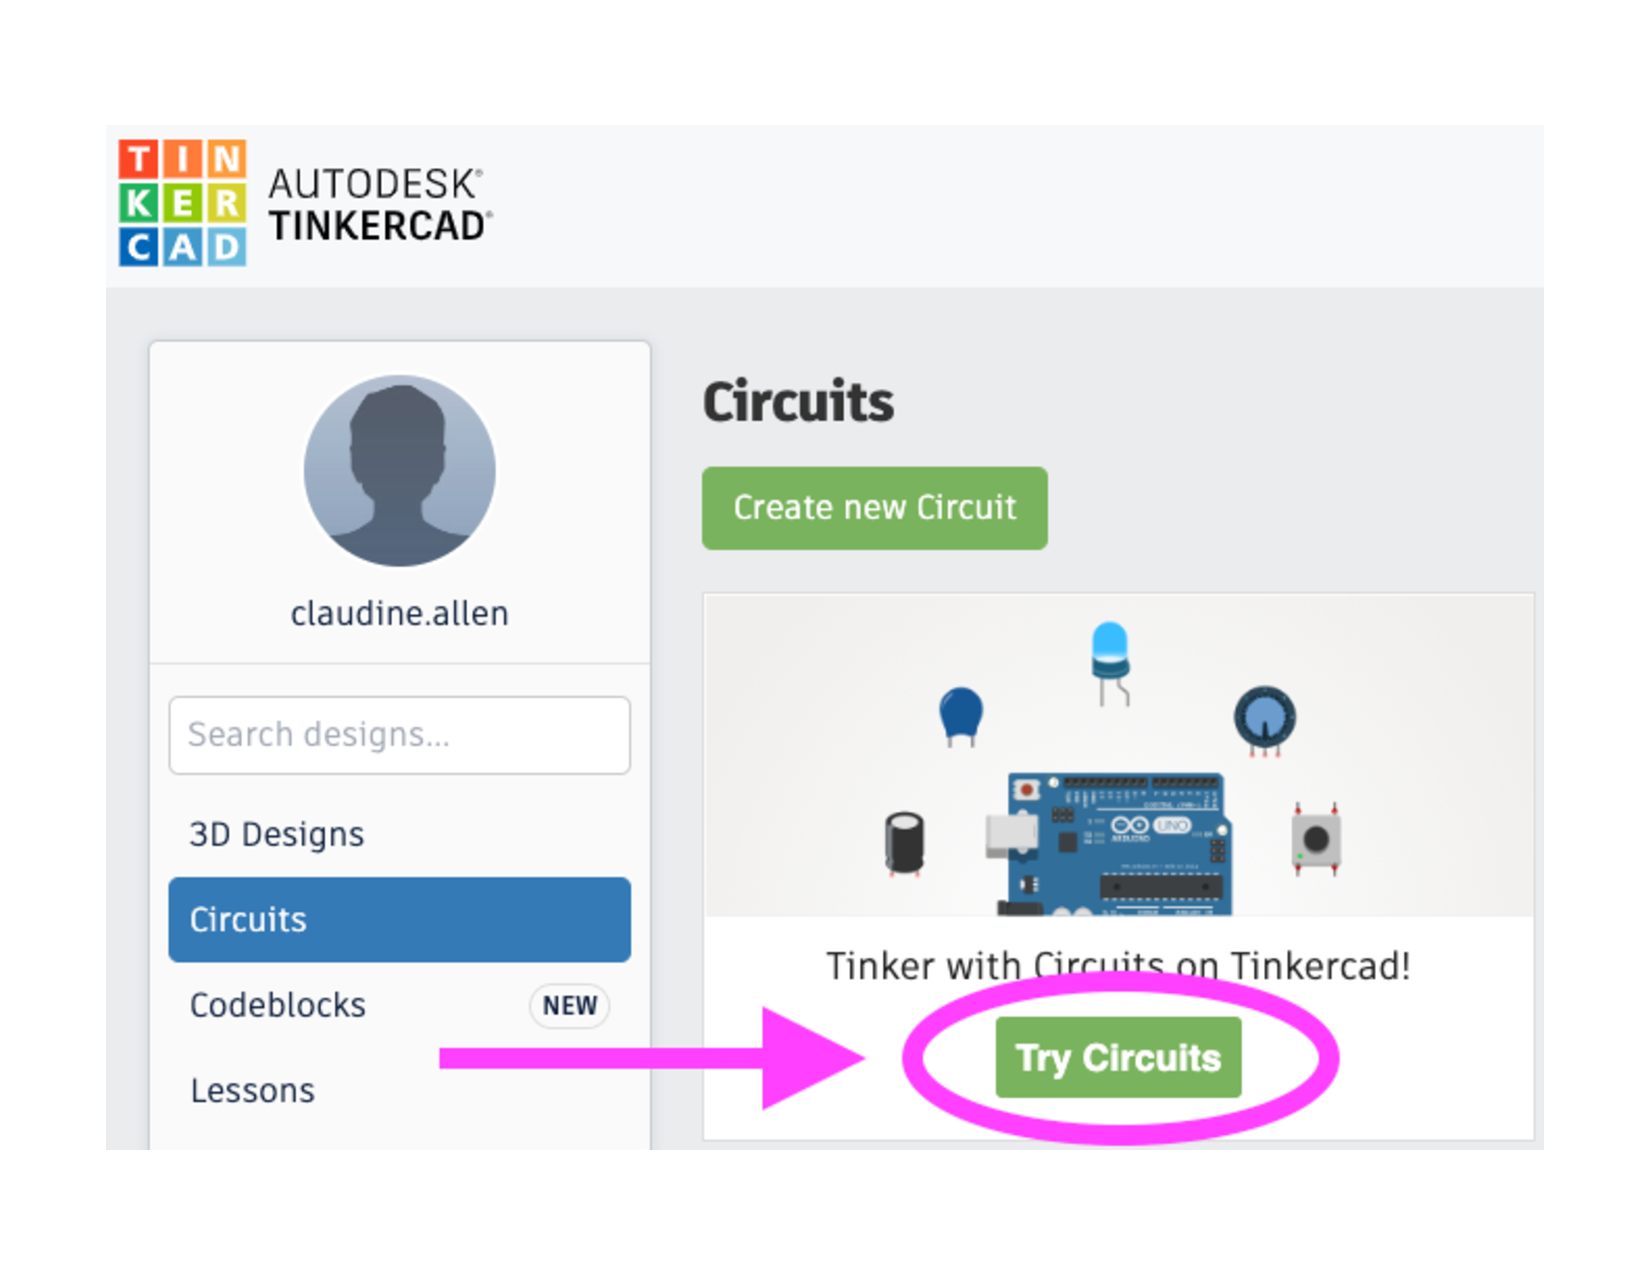
\includegraphics[width=.5\linewidth]{Tutoriel_Circuits_TinkerCad.pdf}
%     \caption{Capture d'écran du service infonuagique Tinkercad indiquant où trouver le tutoriel.}
%     \label{fig:tinkercad-trycircuits}
% \end{figure}

% Sur la gauche, vous trouverez la section \texttt{Circuits} rassemblant vos éventuels \texttt{Workspaces} de conception. À l'intérieur de ces derniers, vous pourrez aussi travailler sur vos designs de circuits en commun à l'aide du bouton \texttt{Share}.

% Complétez le tutoriel dans cette section, sans aucune note à prendre, en cliquant sur le bouton vert \texttt{Try Circuits} encerclé à la figure~\ref{fig:tinkercad-trycircuits}. Ce tutoriel est constitué de 4 leçons: \texttt{Start Simulating, Editing Components, Wiring Components} et \texttt{Adding Components}. Ce seront donc ces leçons qui seront évaluées individuellement, directement en ligne, pour ensuite faire virtuellement les manipulations du laboratoire sur Tinkercad lorsque vous êtes le.la membre de l'équipe en connexion à distance à la maison.
%Tinkercad et être la maison: mise à jour du 1er  protocole

%\newpage
\section[Matériel]{Matériel\footnote{Des photos accompagnent l'inventaire de composants \& instruments <\url{https://airtable.com/shrdI8Y6AqbNd7tZ8}> pour vous aider à identifier le matériel. Certains éléments, comme la patate(!), vous seront parfois remis au début du laboratoire.}} \label{sec:mat}

\noindent La réalisation de ce laboratoire requiert l'utilisation de:
\vspace{1ex}
\begin{itemize} \itemsep5pt
\item une plaquette de montage (\textit{breadboard});
\item un multimètre à 4\textonehalf~chiffres;
\item un multimètre à 6\textonehalf~chiffres;
\item un module d'acquisition NI USB-6008;
\item un ordinateur avec le logiciel \textit{LabVIEW};
\item un adaptateur de charge courant alternatif à courant continu (CA/CC);
\item une pomme de terre;
\item quatre tiges métalliques qui serviront d'électrodes pour la patate : aluminium, zinc, acier, acier inoxydable (Pour éviter toute confusion avec l'acier, le terme «inox» sera utilisé dorénavant pour désigner «acier inoxydable».);
\item deux résistances électriques (nominalement 12~$\Omega$ et 1~k$\Omega$);
\item une pile électrique 9~V.
\end{itemize}

\section{Manipulations} \label{sec:manip}

\setlength{\parskip}{1ex plus 0.5ex minus 0.2ex}

%REPORTER AU LAB II \subsection{Partie 0 --- Exercice de statistiques en métrologie}

%Pendant la présentation introduisant des notions de base et un peu d'historique en métrologie, vous serez conviés à mesurer les dimensions d'une efface et estimer son volume avec 2 outils étalonnés. Ces mesures expérimentales seront rassemblées pour illustrer quelques concepts de statistiques et métrologie en fin de présentation.


\subsection{Partie 1 --- VI \textit{LabVIEW} contrôlant le module d'acquisition}

Tout au long de la création du VI \textit{LabVIEW}, n'oubliez pas d'enregistrer souvent votre fichier. À moins que vous ne teniez à tout recommencer du début\dots

a) Après vous être procuré le matériel complémentaire, soit une pomme de terre, quatre tiges et le module d'acquisition, branchez ce dernier dans un port USB de l'ordinateur.

b) Démarrez le logiciel \textit{LabVIEW} et ouvrez un VI vide. Faites \texttt{Ctrl+E} pour afficher le diagramme ainsi que la face-avant si une seule de ces deux interfaces est ouverte initialement. Le raccourci \texttt{Ctrl+H}, quant à lui, affiche une fenêtre d'aide contextuelle à laisser ouverte et consulter tout au long du développement de votre VI.

c) Sur le diagramme, affichez la palette \textbf{Fonctions} à l'aide d'un clic droit et sélectionnez l'\textbf{Assistant DAQ} (\texttt{Fonctions $\rightarrow$ Express $\rightarrow$ Entrée $\rightarrow$ Assistant DAQ}). Placez l'Assistant DAQ sur le diagramme. Il se lancera automatiquement et la boîte de dialogue \textbf{Créer un nouvel objet Tâche Express} apparaîtra. Dans celle-ci, sélectionnez \texttt{Acquérir des signaux $\rightarrow$ Entrée analogique $\rightarrow$ Tension}. Sélectionnez la voie \textbf{ai0} et cliquez sur \textbf{Terminer}.

L'Assistant DAQ ouvrira ensuite une nouvelle boîte de dialogue qui affiche les options de configuration d'une boucle While pour la voie sélectionnée. Sous l'onglet \textbf{Configuration}, vous pouvez renommer la voie \textbf{ai0} avec un clic droit pour ainsi titrer la série de données de votre acquisition. Remarquez aussi l'endroit où sont définies les valeurs de tension minimale ($v_{min}$) et maximale ($v_{max}$) de la plage permise pour le signal d'entrée. Au bas de la page, changez le mode d'acquisition pour \textbf{Échantillons continus}, changez le nombre d'\textbf{Échantillons à lire} pour 10 et mettez une \textbf{Fréquence} de $f=10$~Hz. Ceci signifie qu'à chaque itération le module acquerra 10~données et qu'il y aura 10~données prises à chaque seconde (donc une itération par seconde). La fréquence $f$ et la plage $[v_{min},v_{max}]$ seront adaptées à chaque mesure de la prochaine partie. Lorsque tout ceci est fait, cliquez sur \textbf{OK}. Une boîte de dialogue \textbf{Confirmer la création automatique de la boucle} apparaîtra. Cliquez sur \textbf{Oui} et \textit{LabVIEW} créera automatiquement une boucle While autour du VI.

Si vous avez correctement cliqué sur \textbf{Oui}, allez maintenant à l'étape d). Si vous avez cliqué sur \textbf{Non} (malheur!), vous devrez rajouter une boucle While manuellement. Pour ce faire, sélectionnez une boucle While (\texttt{Fonctions $\rightarrow$ Programmation $\rightarrow$ Structures $\rightarrow$ Boucle While}) et placez-la sur le diagramme de façon à ce qu'elle englobe l'Assistant DAQ (faites-la plus grande que nécessaire, d'autres objets devront être placés à l'intérieur de la boucle). Maintenant, rajoutez un bouton Stop. Pour ce faire, allez à la face-avant (\texttt{Ctrl+E}), ajoutez-y un bouton-poussoir (\texttt{Commandes $\rightarrow$ Moderne $\rightarrow$ Booléen $\rightarrow$ Bouton-poussoir}) puis changez son nom pour \texttt{Stop}. Par la suite, retournez au diagramme ; vous constaterez que le bouton \texttt{Stop} a été rajouté. Déplacez-le à l'intérieur de votre boucle While s'il n'y est pas déjà. Reliez la sortie du bouton \texttt{Stop} à l'entrée \textbf{stop~(F)} de l'Assistant DAQ et reliez la sortie \textbf{arrêtée} de l'Assistant DAQ au terminal de condition de la boucle While (l'octogone rouge). Vous pouvez agrandir l'icône de l'Assistant DAQ afin de mieux voir ses entrées et ses sorties.

d) Sur le diagramme, cliquez avec le bouton droit sur la sortie \textbf{Données} et sélectionnez \texttt{Créer $\rightarrow$ Indicateur graphe}. Un graphe apparaît sur la face-avant. Sur le diagramme, si l'indicateur graphe est placé à l'intérieur de la boucle While, celui-ci affichera les valeurs mesurées en continu. S'il est placé en-dehors de la boucle, alors il affichera l'ensemble des valeurs lorsque toutes les itérations auront été faites. Puisqu'on souhaite ce dernier type de graphique, placez l'indicateur en-dehors de la boucle (mais veillez à ce qu'il soit tout de même relié à l'aide d'un fil à la sortie \textbf{données} de l'Assistant DAQ).

e) Il serait intéressant d'avoir aussi des indicateurs qui afficheraient les valeurs mesurées pendant l'exécution du VI, pour voir si tout fonctionne correctement. Pour ce faire, encore sur la sortie \textbf{Données}, créez un indicateur numérique. Cet indicateur doit être placé dans la boucle pour avoir l'effet escompté. L'indicateur d'itération, quant à lui, se crée en cliquant avec le bouton droit sur le terminal d'itération, soit le carré bleu \textbf{i} représentant la variable qui contient la valeur de l'itération en cours.

f) Maintenant que le VI peut mesurer une tension et afficher les résultats en continu, il ne reste qu'à le configurer afin qu'il enregistre les résultats automatiquement dans un fichier sur l'ordinateur. Ajoutez la fonction \textbf{Écrire dans un fichier de mesures} (\texttt{Fonctions $\rightarrow$ Programmation $\rightarrow$ E/S sur fichiers $\rightarrow$} \texttt{Écrire dans un fichier de mesures}) et placez-le dans la boucle While, à droite de l'Assistant DAQ (vous pouvez agrandir la boucle au besoin). La boîte de dialogue \textbf{Configurer Écrire dans un fichier de mesures} apparaît. Le champ \textbf{Nom de fichier} affiche l'endroit où les mesures seront enregistrées sur un ordinateur, incluant le chemin complet dans l'arborescence du système de fichiers \href{https://docs.python.org/3/library/pathlib.html}{souvent nécessaire au traitement} et à l'analyse des données informatiques. Modifiez ce champ avec un nom de fichier simple et représentatif en incluant la date. Vous avez même l'option d'ouvrir une boîte de dialogue pour modifier ce nom à chaque fois que le VI est exécuté en cochant l'option \textbf{Demander à l'utilisateur de choisir un fichier}. Aussi, n'ayez pas peur de l'extension~\texttt{.lvm}: il s'agit d'un simple fichier texte.

Dans la section \textbf{Si le fichier existe déjà}, cochez l'option \textbf{Incrémenter le nom du fichier}. Dans la section \textbf{En-têtes de segment}, cochez \textbf{Un seul en-tête}. Cliquez sur \textbf{OK} lorsque tout est fait. Reliez la sortie \textbf{Données} de l'Assistant DAQ à l'entrée \textbf{Signaux} de l'icône \textbf{Écrire dans un fichier de mesures}.

g) Pour tester votre VI, placez la face-avant côte à côte avec le diagramme et \texttt{Animez l'exécution} du flux des données informatiques en appuyant sur le bouton montrant une ampoule au haut de ce dernier, près du bouton avec la flèche démarrant l'exécution. Lancez donc cette exécution et lorsque vous êtes convaincus.es que tout fonctionne bien, appuyez sur le bouton \texttt{Stop} puis désactivez l'animation des données qui est pratique pour le débogage, mais ralentit l'exécution du VI. Accélérez aussi la \textbf{Fréquence} d'échantillonage à $f=100$~Hz dans l'Assistant DAQ.

%%Une tcolorbox serait encore plus sympa pour ça :) :)
\vspace{1ex}
\noindent\framebox{\parbox{\dimexpr\linewidth-2\fboxsep-2\fboxrule}{\textbf{Sagesse expérimentale:} Vérifier immédiatement que les données sont bien enregistrées dans le fichier après chaque exécution vous évitera bien des mots de tête. Cela peut se faire rapidement à l'aide d'un simple éditeur de texte, par exemple \textit{Bloc-notes (Notepad)} sur \textit{OS Windows} ou \textit{TextEdit} sur \textit{MacOS}. Un esprit critique attentif pourra même parfois déjà déceler des erreurs de mesures problématiques. Par exemple, une colonne entière de valeurs très proches de zéro peut être suspecte si le signal mesuré n'est pas censé être nul.}} 
\vspace{1ex}

h) Rajoutez maintenant un script qui arrêtera automatiquement le processus après 1000 mesures. Pour ce faire, rajoutez une constante numérique (\texttt{Fonctions $\rightarrow$ Programmation $\rightarrow$ Numérique $\rightarrow$ Constante numérique}) et placez-la dans la boucle While, près du terminal d'itération. Fixez la constante à 100 (puisque 1000 mesures correspondent à 100 itérations). Ensuite, insérez une commande de comparaison \texttt{Supérieur ou égal} (\texttt{Fonctions $\rightarrow$ Programmation $\rightarrow$ Comparaison $\rightarrow$ Supérieur ou égal~?}). Reliez le terminal d'itération \textbf{i} et la constante numérique aux entrées $x$ et $y$ respectivement de la fonction \texttt{Supérieur ou égal}, afin que le résultat soit faux lorsque $\mathbf{i}<constante$. Maintenant, supprimez le fil qui relie le bouton Stop à l'Assistant DAQ. Puis, reliez la sortie de la fonction \texttt{Supérieur ou égal} et la sortie du bouton \texttt{Stop} aux entrées d'une fonction \texttt{OU} (\texttt{Fonctions $\rightarrow$ Programmation $\rightarrow$ Booléen $\rightarrow$ OU}). Enfin, reliez la sortie du \texttt{OU}  à l'entrée \textbf{stop~(F)} de l'Assistant DAQ. Ainsi, l'acquisition de données s'arrêtera lorsque 100 itérations auront été faites (soit 1000 mesures) ou lorsque l'utilisateur appuiera sur le bouton Stop.
\newpage
i) Étant donné la résolution peu élevée des modules d'acquisition NI USB-6008 pour les signaux électriques peu bruyants à mesurer dans la partie suivante, un signal bruyant de référence sera utile pour l'analyse des expériences. Pour faire générer par \textit{LabVIEW} une forme d'onde avec une distribution aléatoire de bruit blanc gaussien, insérez \texttt{Fonctions $\rightarrow$ Traitement du signal $\rightarrow$ Génération wfm $\rightarrow$ Wfm gauss} dans la boucle While. En entrée \textbf{Infos sur l'éch}(antillonage) de cette forme d'onde, créez une constante avec les valeurs 100~Hz et 10 qui sont alors respectivement identiques à la fréquence et au nombre d'échantillons de chaque série de mesures de tension du module. Entrez aussi une valeur de 0.001 pour l'\textbf{écart type}. Reliez le \textbf{Signal en sortie} de la forme d'onde à l'entrée \textbf{Signaux} de l'icône \textbf{Écrire dans un fichier de mesures}. \textit{LabVIEW} devrait alors proposer automatiquement d'\texttt{Assembler des signaux} dans une seule entrée, sinon cela se trouve dans \texttt{Fonctions $\rightarrow$ Express $\rightarrow$ Manipulation de signaux $\rightarrow$ Assembler}.

j) Le VI est maintenant terminé. Si ce n'était pas déjà fait, enregistrez-le! S'il vous reste des fils brisés, enlevez-les avec \texttt{Ctrl+B}, puis assurez-vous que votre VI soit le plus clair possible avec \texttt{Ctrl+U} et en déplaçant manuellement les fils et objets au besoin.


\subsection{Partie 2 --- Mesures en tension de sources d'alimentation}

Avant d'étudier les sources d'alimentation électrochimiques que sont la patate et la pile, vous ferez l'acquisition de données de tension pour les cas opposés de circuit ouvert avec et sans adaptateur CA/CC. N'hésitez pas à amener de vieux chargeurs inutiles de chez vous qui font cette rectification CA~$\rightarrow$~CC, tant que leur sortie de courant continu (\textit{direct current, DC}) fournit une tension inférieure à 10~V. Vous pourrez alors les ouvrir à la fin du laboratoire, avec l'assistance de notre merveilleuse équipe technique, pour voir comment ils sont faits à l'intérieur! Mais d'abord:

a) À l'aide du multimètre à 4\textonehalf~chiffres, de fils bananes et de pinces crocodiles, mesurez la différence de potentiel entre les bornes d'un adaptateur CA/CC. Il s'agit ici de votre premier résultat de mesure expérimentale à écrire dans votre cahier de recherche, celui-ci comme tous les autres à venir doit comporter une estimation de l'incertitude et des explications justifiant les causes de cette dernière.

b) Branchez ensuite les deux fils de l'adaptateur CA/CC dans les trous des \textit{rails} d'alimentation positive et négative d'une plaquette de montage. En respectant la polarité (direction d'un éventuel courant dans ce contexte), insérez ensuite dans ces mêmes \textit{rails} le fil rouge sortant de la borne $+$ et celui noir de la borne $-$ du module d'acquisition à sa voie \textbf{ai0}.

c) Dans le VI que vous avez construit en première partie, retournez à l'Assistant DAQ pour modifier la plage du signal d'entrée entre $[0,v_{max}]$ afin de couvrir la valeur de tension CC spécifiée sur l'adaptateur. Une pratique empirique est de placer le signal aux environs des $3/4$ de la plage. Réalisez alors une acquisition de données numériques avec le module branché. 

d) Transférez le fichier \texttt{.lvm} obtenu dans votre canal privé MS Teams via l'onglet correspondant accompagnant votre cahier de recherche. Notez que le crochet dans la fenêtre de transfert génère une publication et des notifications intempestives, à éviter svp\footnote{Vous pouvez aussi transférer tous vos fichiers pour le travail à distance seulement à la fin du laboratoire, mais n'oubliez pas de le faire, car l'ordinateur peut être réinstallé en effaçant les données à tout moment.}. Il s'agit ici de votre premier enregistrement d'un signal de mesures à consigner dans votre cahier de recherche, n'oubliez jamais d'indiquer le chemin complet et le nom du fichier de ces données pour le retrouver facilement à son endroit de stockage final. Notez aussi les conditions expérimentales et les paramètres de mesure, comme la plage de tension du module, ainsi que toute observation pertinente, en particulier des effets systématiques qui pourraient nuire à la justesse du résultat de mesure ainsi que des pistes de solution pour éliminer ces erreurs systématiques. Cette étape ne sera plus mentionnée du reste du cours, mais il va de soi qu'elle doit être répétée après chaque acquisition de données.

e) Débranchez l'adaptateur et refaites la même acquisition, mais cette fois-ci avec une plage de tension d'entrée [-1,1]~V pour la mesure. Supprimez ensuite la fonction générant la forme d'onde bruyante (\textbf{Wfm gauss}) dans le diagramme du VI et enlevez les fils brisés avec \texttt{Ctrl+B}, car cette référence de bruit ne sera plus nécessaire pour le reste du laboratoire.
 
f) Abandonnant temporairement la plaquette de montage pour travailler avec la pomme de terre, insérez-y les tiges d'inox et d'aluminium de manière à avoir une distance de quelques centimètres entre les deux. Enfoncez-les bien. %Faites attention de ne pas manger la patate ; cela viendrait fausser les résultats.

g) Mesurez la différence de potentiel entre les deux électrodes (les tiges à connecter en matériaux de différentes électronégativités) avec le multimètre à 4\textonehalf~chiffres, puis modifiez la tension $v_{max}$ en entrée dans l'Assistant DAQ de votre VI à une valeur appropriée.

h) Utilisez exceptionnellement juste les pinces alligators pour faire tenir les fils de la voie \textbf{ai0} du module d'acquisition en contact avec les électrodes d'inox et d'aluminium, puis exécutez le VI en prenant toujours soin d'examiner brièvement le fichier de données enregistré à la fin. 

i) Échangez les tiges pour une combinaison d'électrodes acier--aluminium puis faites une nouvelle acquisition de tension.

j) Retournez finalement à la plaquette de montage pour y brancher la pile de 9~V ainsi que le module d'acquisition dans les \textit{rails} d'alimentation et lancez votre VI avec une valeur d'entrée $v_{max}$ appropriée. 

\subsection{Partie 3 --- Conversion en courant}

Toutes les mesures effectuées jusqu'à maintenant étaient simplement aux bornes de sources d'alimentation, donc en circuit ouvert sans courant significatif qui circule. Les expériences du laboratoire se concluent donc en fermant le circuit avec des charges résistives pour mesurer le courant circulant dans la maille.

\begin{figure}[h]
\centering
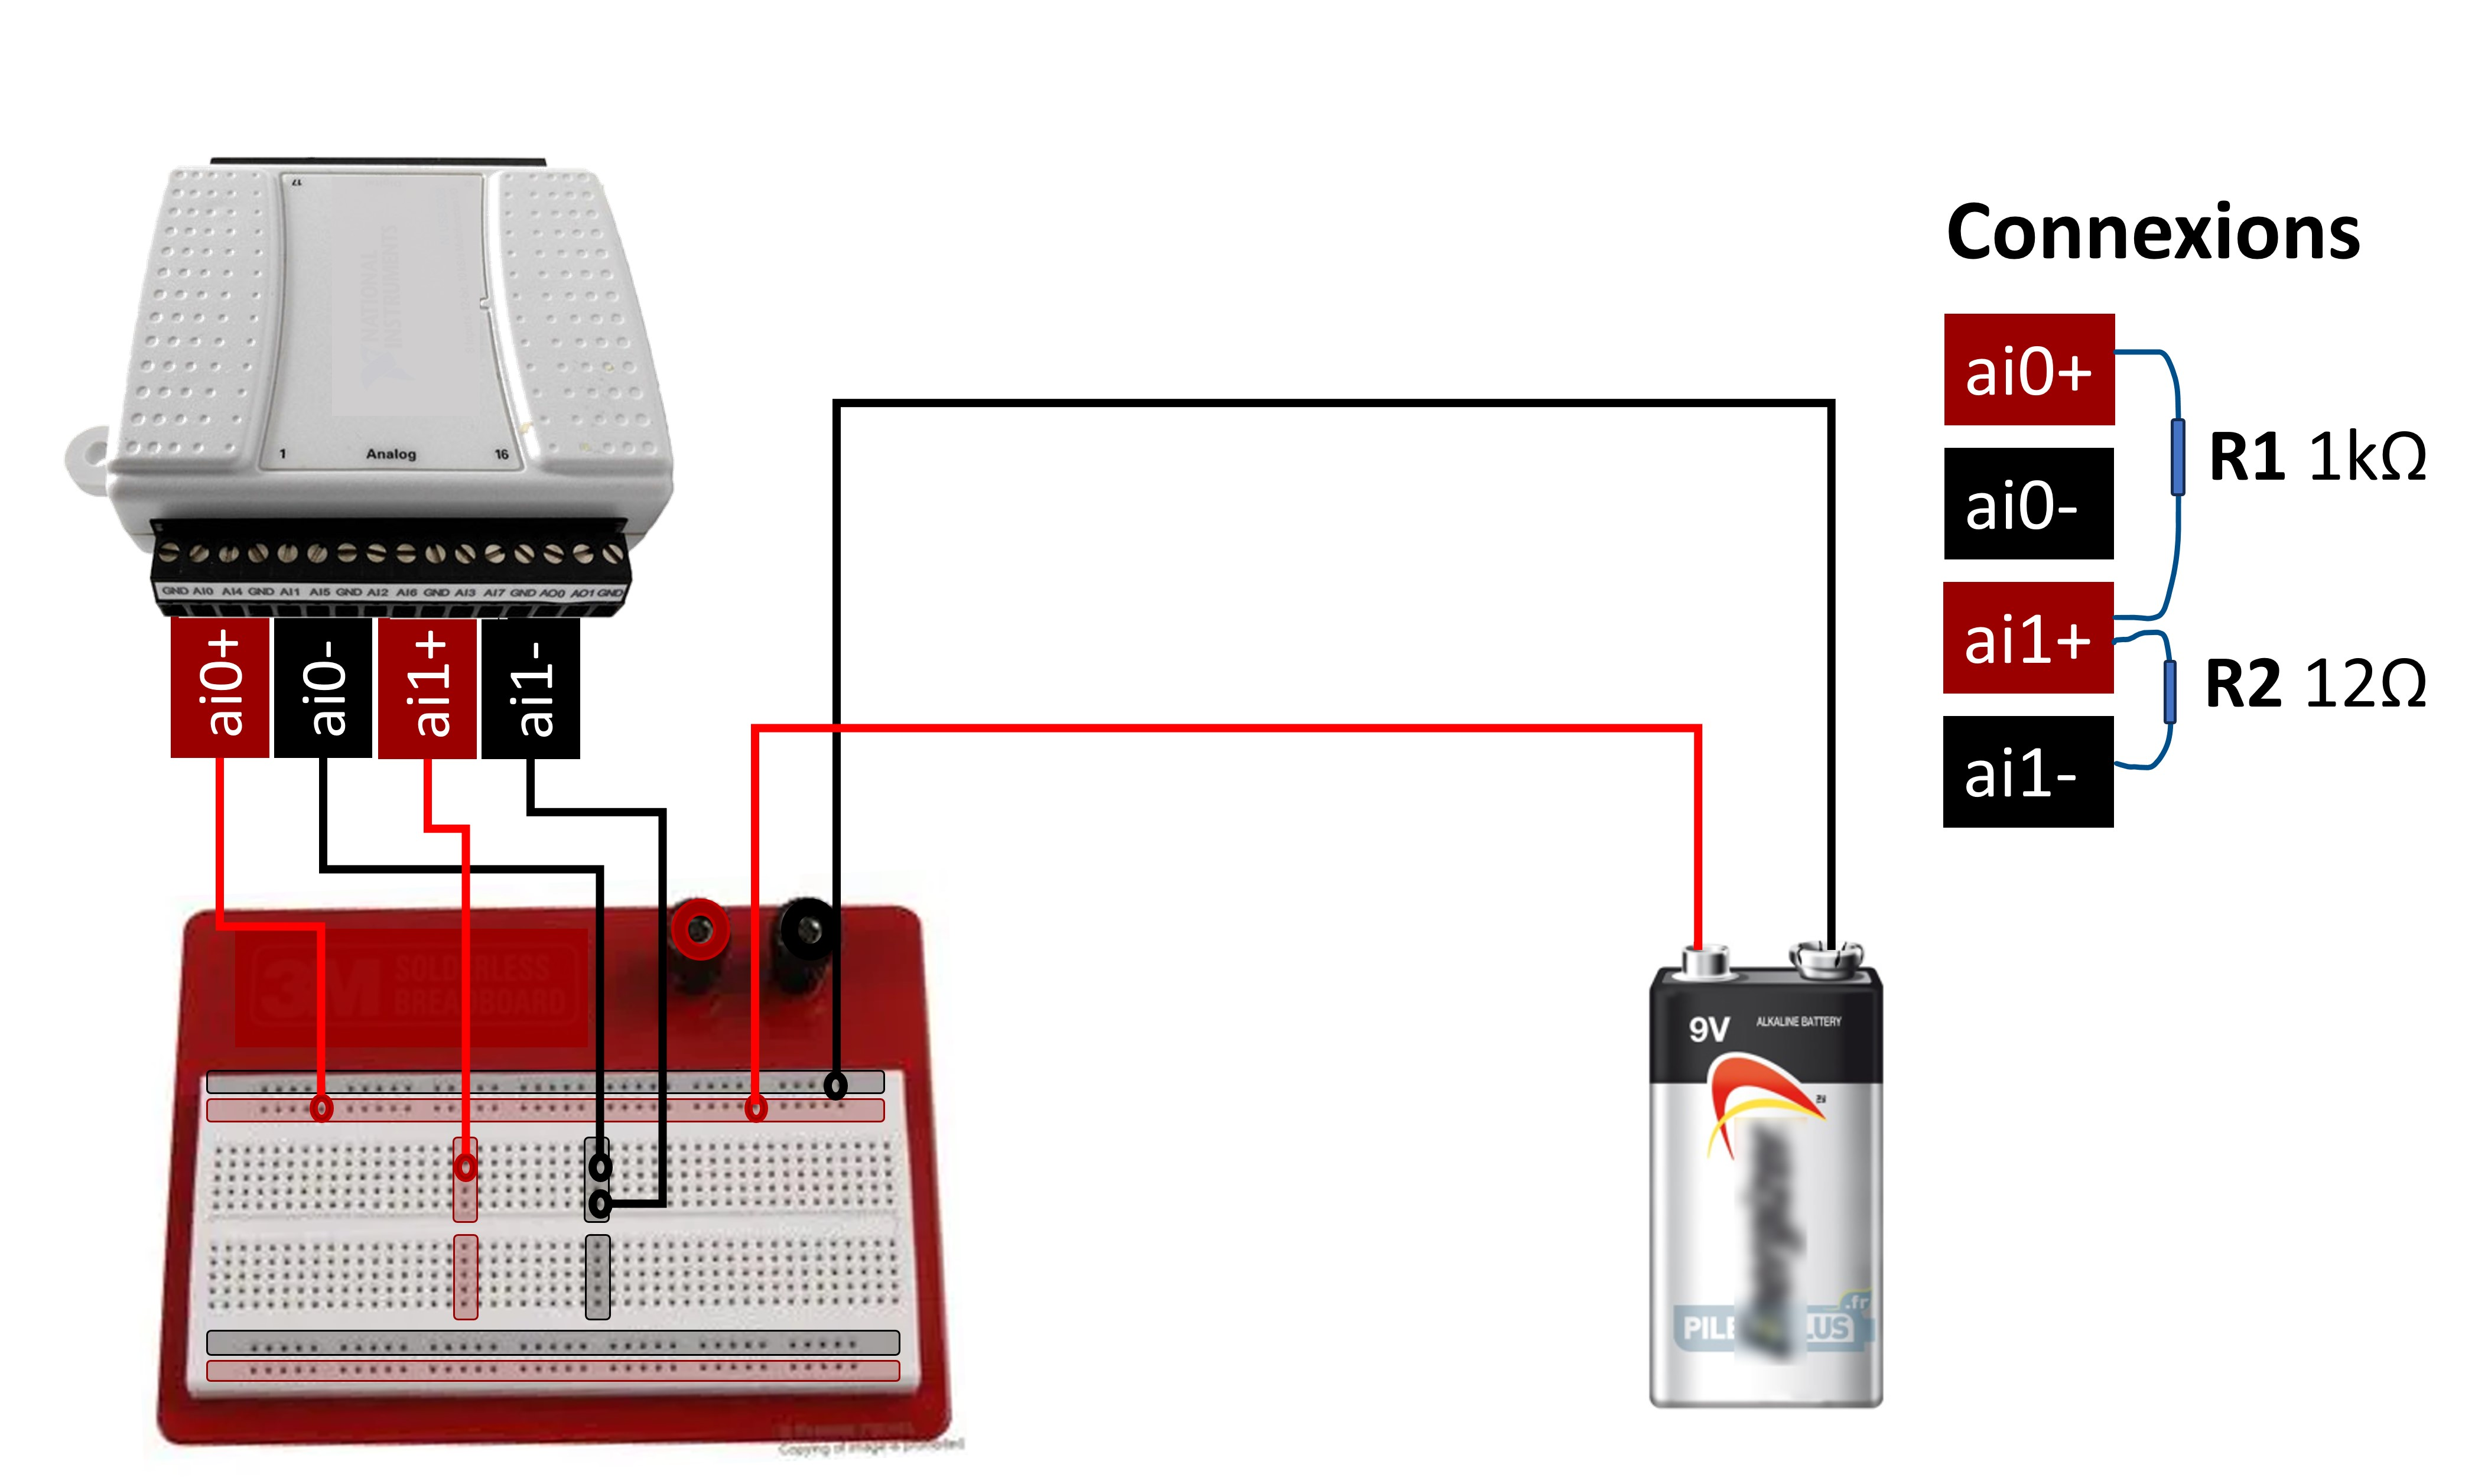
\includegraphics[width=0.9\textwidth]{L01-sch-poweredbreadboard}
\caption{\label{L01-sch-poweredbreadboard} Illustration pour aider à réaliser le premier circuit fermé sur la plaquette de montage avec R1~=~1~k$\Omega$ et R2~=~12~$\Omega$.}
\end{figure}

a) Sur votre plaquette déjà alimentée par la pile de 9~V, connectez cette dernière à une résistance de 1~k$\Omega$ en série avec une résistance de 12~$\Omega$. De plus, reliez les bornes de la petite résistance à l'entrée \textbf{ai1} du module d'acquisition comme illustré à la figure~\ref{L01-sch-poweredbreadboard}. La mesure de la tension aux bornes de cette résistance de 12~$\Omega$ permettra de calculer le courant circulant dans le circuit maintenant fermé.

b) Modifiez votre VI afin qu'il puisse acquérir simultanément deux mesures de tension. Pour ce faire, allez dans les propriétés de l'Assistant DAQ et rajoutez une voie. Sélectionnez \textbf{Tension} puis \textbf{ai1} et faites \textbf{OK}. Prenez les mêmes paramètres que pour la voie \textbf{ai0} et cliquez sur \textbf{OK}.

c) Faites une acquisition des données numériques en exécutant une dernière fois le VI.

d) Pour appliquer la loi d'Ohm avec votre logiciel d'analyse numérique choisi, divisez par 12~$\Omega$ les valeurs de tension enregistrées pour la voie \textbf{ai1} afin de calculer le courant\footnote{Négligez l'incertitude de la résistance de 12~$\Omega$ pour ce calcul.}. Vous avez alors l'équivalent d'un (mauvais) ampèremetre puisque ce courant calculé est le même qui traverse la plus grosse résistance. %Très moyen d'avoir ça pitché ici vu que dans cette nouvelle version du protocole, l'analyse numérique et graphique commence à se faire seulement à la section suivante.

\subsection{Début d'analyse de la partie 2 directement au laboratoire}
Il est fortement recommandé de commencer à traiter et visualiser ses données expérimentales avant de quitter cette première séance de laboratoire. Vous bénéficierez alors du support de l'équipe d'enseignement en se lançant dans votre analyse avec de nouveaux outils informatiques d'analyse.

\begin{itemize}
    \item Consultez les consignes à appliquer pour tout graphique, elles sont données dans le module de cours 2 de la section "Contenu et activités" sur notre site.
    \item En ignorant la colonne de référence de bruit pour l'instant dans vos 2 premiers fichiers \texttt{.lvm}, faites un graphique\footnote{Le choix de logiciel n'est pas imposé à ce point-ci, mais une liste de possibilités recommandées se retrouve aussi dans le module de cours 2. Il est recommandé d'évoluer progressivement vers les outils du langage \textit{Python} libre d'accès et bien adapté aux travaux de physique. L'équipe d'enseignement peut vous conseiller dans ce choix en fonction de votre niveau actuel de connaissances informatiques.} de la tension en nuages de points (\textit{scatter}) pour chaque source de la partie 2 et ajoutez à chaque graphique les données de référence d'un signal nul mesuré à l'étape e) de cette partie. Notez que l'abscisse des graphiques est simplement le numéro d'index de la mesure et non pas strictement en fonction du temps, car nous n'avons pas inclus de fonctions dans notre VI pour interroger les horloges du module d'acquisition et de l'ordinateur.
    \item Les graphiques où la tension fluctue, mais ne varie pas significativement dans le temps sont dans un régime dit (statistiquement) stationnaire, d'où l'acquisition de données devient équivalente à répéter la même mesure. Pour ces graphiques, évaluez numériquement la moyenne de tension $\Bar{v}$ fournie par la source ainsi que sa variance $\sigma_v^2$.
    \item Le rapport signal sur bruit, $SNR$, se définit en prenant le ratio du carré de la moyenne sur la variance, \textit{i.e.} \(\displaystyle SNR\equiv \frac{\Bar{v}}{\sigma_v^2}\). Calculez ce rapport avec les moyennes et variances obtenues au point précédent pour les sources en régime stationnaire et déterminez laquelle a le meilleur SNR.
    %Ajouter un/des paramètres associés à la matrice de covariance pour caller la nonstationnarité. Idéalement lier à corrélation n'est pas causation.
    \item Comparez graphiquement les deux séries de mesures de l'étape e), donc en incluant le signal bruyant généré par \textit{LabVIEW}. Observez aussi ces données sous forme d'histogramme, \textit{i.e.} en représentant en colonnes le nombre de données mesurées par intervalle de tension. Ajustez le nombre d'intervalles afin d'obtenir un histogramme significatif: trop ou trop peu d'intervalles ne permettent pas de bien voir la distribution statistique des données.
\end{itemize}

%Partie 3 : Pour appliquer la loi d'Ohm avec votre logiciel d'analyse numérique choisi, divisez par 12~$\Omega$ les valeurs de tension enregistrées pour la voie \textbf{ai1} afin de calculer le courant\footnote{Négligez l'incertitude de la résistance de 12~$\Omega$ pour ce calcul.}. Vous avez alors l'équivalent d'un (mauvais) ampèremetre puisque ce courant calculé est le même qui traverse la plus grosse résistance.

%NE PAS OUBLIER DE RÉVISER LA QUESTION D'ANALYSE DE BIAIS DE MESURE DU LAB II

%...) Si le temps le permet, n'hésitez pas à ... plus de tiges, pile usée vs pile neuve etc. la créativité va ici :)

\vspace{-0.5cm}
\section[Questions d'analyse I]{Questions d'analyse I\footnote{Pour cultiver de bonnes habitudes d'intégrité en recherche, les expériences échouées devront être reprises quitte à retourner au laboratoire VCH-0647 accessible en tout temps, soit exactement ce que vous feriez en milieu de travail professionnel. Les données et mesures d'autres équipes ne doivent donc pas être plagiées (professionnellement, ce serait alors une fraude scientifique) à moins d'une très rare autorisation des titulaires de cours; la provenance des données devra alors être explicitement citée pour éviter le plagiat. Pour compléter la sagesse expérimentale encadrée précédemment, il est alors clair que quelques vérifications préliminaires de vos données avant de quitter la séance de laboratoire, dans l'esprit d'arriver à bien répondre aux questions d'analyses, pourront vous éviter la perte de temps de recommencer des manipulations par la suite. Lorsque cela s'avère nécessaire malgré tout, le.la technicien.ne attitré.e au cours pourra sortir tout matériel qui n'est pas dans votre coffre le temps de votre travail puis le ranger; ses coordonnées de contact se retrouvent dans la section \texttt{Informations générales} sur la gauche du site de cours.}} \label{sec:grade} 

\vspace{-0.5cm}
\noindent$\rightarrow$ À remettre en équipe sur \href{https://www.gradescope.com/}{Gradescope} en ajoutant votre \href{https://help.gradescope.com/article/m5qz2xsnjy-student-add-group-members}{binôme de laboratoire} $\leftarrow$

%New QAs ->  QUALITÉ D'UTILISATION INSTRUMENT -> MULTIMÈTRE POUR PATATE VS POWER ADAPTER, PERMET QUESTION ANALYSE SUR QUEL CAS APPROPRIÉ DE PRENDRE MULTIMÈTRE!  Avec les 2 résultats de mesure de multimètre, prep le terrain moitié plus petite incertitude marche pas, manufacturier et autre causes que l'instrument, p-e voir pour mettre la capsule de simon et daniel au lab II. Mais surtout ne pas oublier de faire une question de choix d'instrument tenant compte de la non stationnarité.

\begin{gradescope}
\item Évaluez la résolution de numérisation (conversion analogique-numérique, échantillonnage) du module d'acquisition lors d'une mesure de tension pour le plus petit intervalle utilisé pendant le laboratoire, sachant que cette mesure est une différence (\textit{differential}) de potentiel entre deux points du circuit.\\ \textit{\footnotesize N.B. On fait appel à vos capacités de chercheur, dans le sens littéral de chercher par vous-même, pour comprendre le rôle du module d'acquisition avec son manuel et autres sources d'information (\emph{e.g.} dictionnaire!) sur la numérisation. Des discussions à ce sujet avec l'équipe d'enseignement et sur la chaîne de \texttt{Questions} du \texttt{Teams} de cours sont encouragées.}
    \begin{gradescope}
    \item Quelle est la résolution calculée pour l'intervalle de \qty{-1}{\volt} à \qty{1}{\volt}?
        \begin{itemize}[label=$\blacktriangleright$]
        \item \qty{490}{\mV}
        \item \qty{49}{\mV}
        \item \qty{4.9}{\mV}
        \item \qty{0.49}{\mV}
        \end{itemize}
    \item Avez-vous observé un effet indésirable de cette limite de résolution dans au moins un des graphiques d'analyse pour visualiser vos données? À laquelle des formes suivantes cet effet correspond-il le mieux? $\blacktriangleright$ Triangles $\blacktriangleright$ Rampes $\blacktriangleright$ Paliers %ou marches?
    \end{gradescope}
%\item À l'étape g) de la deuxième partie, vous avez probablement remarqué que la différence de potentiel entre les électrodes dépendait des métaux choisis. Quelle combinaison permet d'obtenir la plus haute tension?
    \begin{gradescope}
    \setcounter{gradescopei}{2}
    \item Avez-vous mesuré une tension qui fluctuait autour de zéro pour la combinaison acier--aluminium? $\blacktriangleright$ Oui $\blacktriangleright$ Non
    \item Si oui, pourquoi en est-il ainsi?
        \begin{itemize}[label=$\blacktriangleright$]
        \item L'acier est oxydé.
        \item Acier et aluminium commencent les deux par la lettre «a», donc ils ne peuvent réagir ensemble.
        \item Les deux métaux ont la même électronégativité.
        \end{itemize}
    \end{gradescope}
%\item Comparez l’histogramme de l’étape~f) pour la combinaison inox-aluminium à celui de l’étape~h) en explicitant en légende lequel des deux correspond le mieux au modèle de la loi normale (distribution gaussienne). Pour le cas où cette loi ne s’applique PAS, présentez aussi graphiquement les données de tension d'une manière différente qui met en lumière le manque de stabilité de la mesure.
\item À partir des mesures de la partie 3 avec la pile en circuit fermé, calculez la valeur de la grosse résistance en utilisant une \textit{évaluation de Type A de l'incertitude} tel que présentée dans l’introduction aux bases de la métrologie. Concrètement, divisez la colonne \textit{tension} par la colonne \textit{courant} pour obtenir une distribution de la mesure de résistance. Puis, comparez la moyenne et la médiane de cette distribution de résistance.%\\ \textit{N.B. Dans cette situation instable, il vaut mieux définir un intervalle d'incertitude très élargi en multipliant par 3 l'écart type~$\sigma$ de votre distribution de données.}
%\item Laquelle ou lesquelles des questions précédentes peuvent être répondues en préparation avant le laboratoire? $\;\blacktriangleright$ Q1.1 $\;\blacktriangleright$ Q1.2 $\;\blacktriangleright$ Q1.3 $\;\blacktriangleright$ Q2.1 $\;\blacktriangleright$ Q2.2 $\;\blacktriangleright$ Q3 $\;\blacktriangleright$ Q4
\item \textsc{Sections de rapport - Introduction \& Conclusion:} Écrivez en moins de 350 mots (combinés) l'introduction et la conclusion d'un rapport scientifique portant sur l'ensemble du laboratoire.\footnote{Les instructions et explications d'écriture pour chaque section sont détaillées dans le document \texttt{Guide de rédaction de rapports scientifiques.}}
\end{gradescope}

\end{document}
OLLLDDDD STUFF!
%\footnote{Explication des \textit{tags} pour chaque numéro:\\
%\texttt{[observation]} : Réponse très courte ou à choix multiple visant à illustrer des commentaires que vous devez apprendre progressivement à remarquer et noter par vous-mêmes dans votre cahier pendant l'expérimentation pour développer votre jugement critique. Il faut réfléchir en manipulant! Cela aide à déceler des problèmes expérimentaux et ainsi développer le premier réflexe de tout chercheur.e et ingénieur.e, soit de modifier et reprendre l'expérience autant de fois que nécessaire.\\
%\texttt{[analyse]} : Résultats présentés selon les règles de présentation et d'écriture en métrologie. L'ensemble de votre réponse doit déjà faire preuve d'analyse critique dans cette étape préliminaire à la rédaction d'un rapport. Par exemple, si vos mesures et observations ont un comportement physiquement inattendu, une courte justification ou hypothèse doit être présentée pour tenter de l'expliquer. Une longue discussion n'est pas requise: la véracité et la qualité priment sur la quantité. Lorsqu'une figure ou un graphique est demandé, il doit respecter les consignes spécifiées dès le début de la page d'introduction du site Internet du cours.\\[-6pt]}